
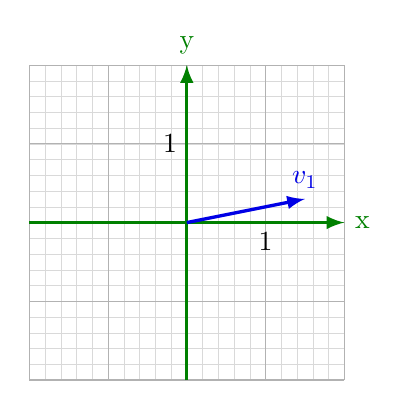
\begin{tikzpicture}[scale=1, samples=100, >=latex]

% Draw the coordinate frame
\def\range{2.}
\draw[step=0.2, very thin,color=gray!30!white] (-\range,-\range) grid (\range,\range);
\draw[step=1.0,color=gray!60!white] (-\range,-\range) grid (\range,\range);
\draw[->, >=latex, very thick, color=green!50!black] (-\range,0) -- (\range,0) node[right] {x};
\draw[->, >=latex, very thick, color=green!50!black] (0,-\range) -- (0,\range) node[above] {y};    
\draw (1, 0) node[left,below]{$1$};    
\draw (0, 1) node[below,left]{$1$};

% draw the vector:
\draw[->,color=blue!90!black, very thick] (0,0) -- (1.5, 0.3) node[above]{$v_1$};
\end{tikzpicture}
